\documentclass[1p]{elsarticle_modified}
%\bibliographystyle{elsarticle-num}

%\usepackage[colorlinks]{hyperref}
%\usepackage{abbrmath_seonhwa} %\Abb, \Ascr, \Acal ,\Abf, \Afrak
\usepackage{amsfonts}
\usepackage{amssymb}
\usepackage{amsmath}
\usepackage{amsthm}
\usepackage{scalefnt}
\usepackage{amsbsy}
\usepackage{kotex}
\usepackage{caption}
\usepackage{subfig}
\usepackage{color}
\usepackage{graphicx}
\usepackage{xcolor} %% white, black, red, green, blue, cyan, magenta, yellow
\usepackage{float}
\usepackage{setspace}
\usepackage{hyperref}

\usepackage{tikz}
\usetikzlibrary{arrows}

\usepackage{multirow}
\usepackage{array} % fixed length table
\usepackage{hhline}

%%%%%%%%%%%%%%%%%%%%%
\makeatletter
\renewcommand*\env@matrix[1][\arraystretch]{%
	\edef\arraystretch{#1}%
	\hskip -\arraycolsep
	\let\@ifnextchar\new@ifnextchar
	\array{*\c@MaxMatrixCols c}}
\makeatother %https://tex.stackexchange.com/questions/14071/how-can-i-increase-the-line-spacing-in-a-matrix
%%%%%%%%%%%%%%%

\usepackage[normalem]{ulem}

\newcommand{\msout}[1]{\ifmmode\text{\sout{\ensuremath{#1}}}\else\sout{#1}\fi}
%SOURCE: \msout is \stkout macro in https://tex.stackexchange.com/questions/20609/strikeout-in-math-mode

\newcommand{\cancel}[1]{
	\ifmmode
	{\color{red}\msout{#1}}
	\else
	{\color{red}\sout{#1}}
	\fi
}

\newcommand{\add}[1]{
	{\color{blue}\uwave{#1}}
}

\newcommand{\replace}[2]{
	\ifmmode
	{\color{red}\msout{#1}}{\color{blue}\uwave{#2}}
	\else
	{\color{red}\sout{#1}}{\color{blue}\uwave{#2}}
	\fi
}

\newcommand{\Sol}{\mathcal{S}} %segment
\newcommand{\D}{D} %diagram
\newcommand{\A}{\mathcal{A}} %arc


%%%%%%%%%%%%%%%%%%%%%%%%%%%%%5 test

\def\sl{\operatorname{\textup{SL}}(2,\Cbb)}
\def\psl{\operatorname{\textup{PSL}}(2,\Cbb)}
\def\quan{\mkern 1mu \triangleright \mkern 1mu}

\theoremstyle{definition}
\newtheorem{thm}{Theorem}[section]
\newtheorem{prop}[thm]{Proposition}
\newtheorem{lem}[thm]{Lemma}
\newtheorem{ques}[thm]{Question}
\newtheorem{cor}[thm]{Corollary}
\newtheorem{defn}[thm]{Definition}
\newtheorem{exam}[thm]{Example}
\newtheorem{rmk}[thm]{Remark}
\newtheorem{alg}[thm]{Algorithm}

\newcommand{\I}{\sqrt{-1}}
\begin{document}

%\begin{frontmatter}
%
%\title{Boundary parabolic representations of knots up to 8 crossings}
%
%%% Group authors per affiliation:
%\author{Yunhi Cho} 
%\address{Department of Mathematics, University of Seoul, Seoul, Korea}
%\ead{yhcho@uos.ac.kr}
%
%
%\author{Seonhwa Kim} %\fnref{s_kim}}
%\address{Center for Geometry and Physics, Institute for Basic Science, Pohang, 37673, Korea}
%\ead{ryeona17@ibs.re.kr}
%
%\author{Hyuk Kim}
%\address{Department of Mathematical Sciences, Seoul National University, Seoul 08826, Korea}
%\ead{hyukkim@snu.ac.kr}
%
%\author{Seokbeom Yoon}
%\address{Department of Mathematical Sciences, Seoul National University, Seoul, 08826,  Korea}
%\ead{sbyoon15@snu.ac.kr}
%
%\begin{abstract}
%We find all boundary parabolic representation of knots up to 8 crossings.
%
%\end{abstract}
%\begin{keyword}
%    \MSC[2010] 57M25 
%\end{keyword}
%
%\end{frontmatter}

%\linenumbers
%\tableofcontents
%
\newcommand\colored[1]{\textcolor{white}{\rule[-0.35ex]{0.8em}{1.4ex}}\kern-0.8em\color{red} #1}%
%\newcommand\colored[1]{\textcolor{white}{ #1}\kern-2.17ex	\textcolor{white}{ #1}\kern-1.81ex	\textcolor{white}{ #1}\kern-2.15ex\color{red}#1	}

{\Large $\underline{11a_{175}~(K11a_{175})}$}

\setlength{\tabcolsep}{10pt}
\renewcommand{\arraystretch}{1.6}
\vspace{1cm}\begin{tabular}{m{100pt}>{\centering\arraybackslash}m{274pt}}
\multirow{5}{120pt}{
	\centering
	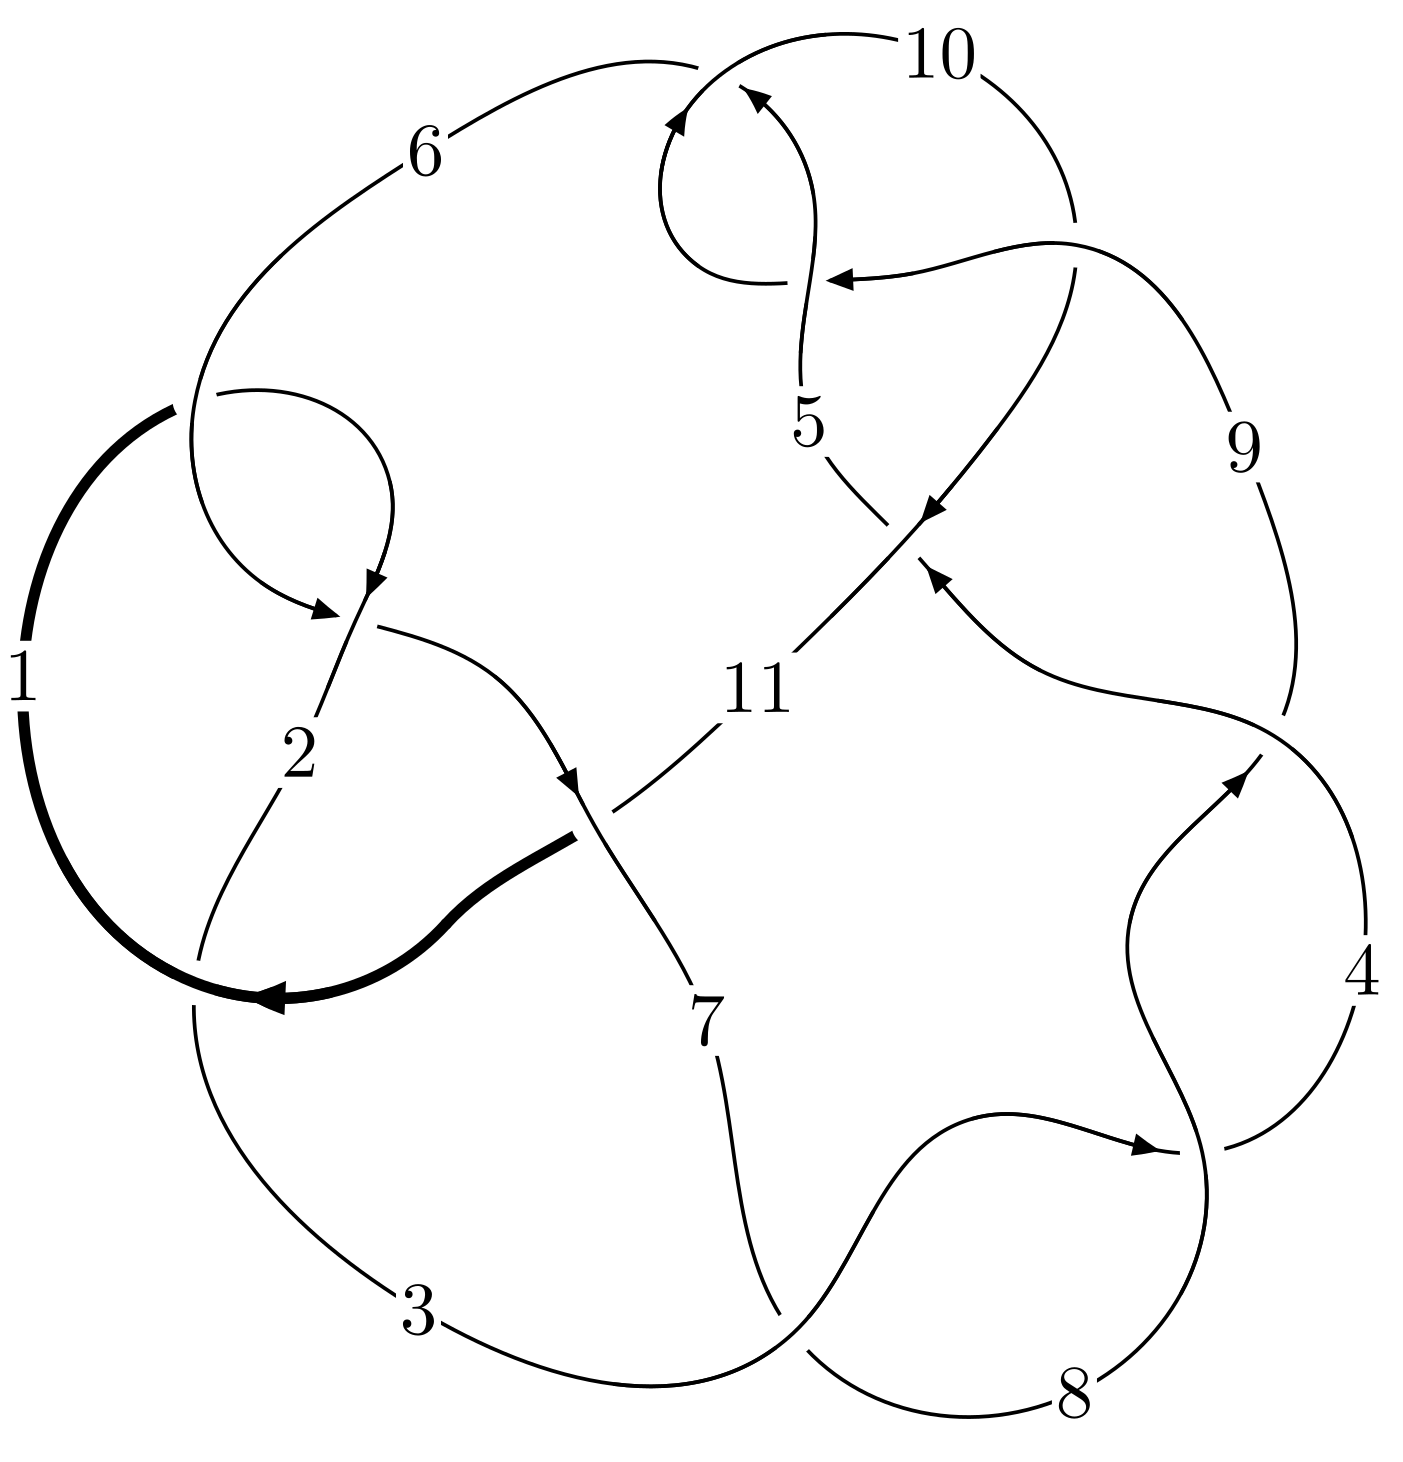
\includegraphics[width=112pt]{../../../GIT/diagram.site/Diagrams/png/424_11a_175.png}\\
\ \ \ A knot diagram\footnotemark}&
\allowdisplaybreaks
\textbf{Linearized knot diagam} \\
\cline{2-2}
 &
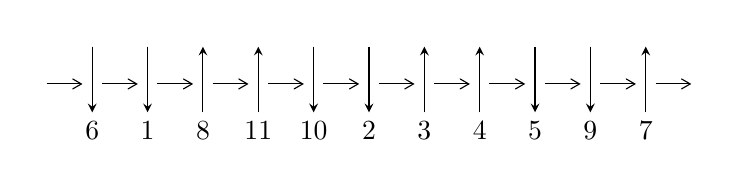
\begin{tikzpicture}[x=20pt, y=17pt]
	% nodes
	\node (C0) at (0, 0) {};
	\node (C1) at (1, 0) {};
	\node (C1U) at (1, +1) {};
	\node (C1D) at (1, -1) {6};

	\node (C2) at (2, 0) {};
	\node (C2U) at (2, +1) {};
	\node (C2D) at (2, -1) {1};

	\node (C3) at (3, 0) {};
	\node (C3U) at (3, +1) {};
	\node (C3D) at (3, -1) {8};

	\node (C4) at (4, 0) {};
	\node (C4U) at (4, +1) {};
	\node (C4D) at (4, -1) {11};

	\node (C5) at (5, 0) {};
	\node (C5U) at (5, +1) {};
	\node (C5D) at (5, -1) {10};

	\node (C6) at (6, 0) {};
	\node (C6U) at (6, +1) {};
	\node (C6D) at (6, -1) {2};

	\node (C7) at (7, 0) {};
	\node (C7U) at (7, +1) {};
	\node (C7D) at (7, -1) {3};

	\node (C8) at (8, 0) {};
	\node (C8U) at (8, +1) {};
	\node (C8D) at (8, -1) {4};

	\node (C9) at (9, 0) {};
	\node (C9U) at (9, +1) {};
	\node (C9D) at (9, -1) {5};

	\node (C10) at (10, 0) {};
	\node (C10U) at (10, +1) {};
	\node (C10D) at (10, -1) {9};

	\node (C11) at (11, 0) {};
	\node (C11U) at (11, +1) {};
	\node (C11D) at (11, -1) {7};
	\node (C12) at (12, 0) {};

	% arrows
	\draw[->,>={angle 60}]
	(C0) edge (C1) (C1) edge (C2) (C2) edge (C3) (C3) edge (C4) (C4) edge (C5) (C5) edge (C6) (C6) edge (C7) (C7) edge (C8) (C8) edge (C9) (C9) edge (C10) (C10) edge (C11) (C11) edge (C12) ;	\draw[->,>=stealth]
	(C1U) edge (C1D) (C2U) edge (C2D) (C3D) edge (C3U) (C4D) edge (C4U) (C5U) edge (C5D) (C6U) edge (C6D) (C7D) edge (C7U) (C8D) edge (C8U) (C9U) edge (C9D) (C10U) edge (C10D) (C11D) edge (C11U) ;
	\end{tikzpicture} \\
\hhline{~~} \\& 
\textbf{Solving Sequence} \\ \cline{2-2} 
 &
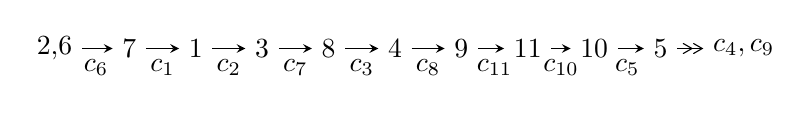
\begin{tikzpicture}[x=24pt, y=7pt]
	% node
	\node (A0) at (-1/8, 0) {2,6};
	\node (A1) at (1, 0) {7};
	\node (A2) at (2, 0) {1};
	\node (A3) at (3, 0) {3};
	\node (A4) at (4, 0) {8};
	\node (A5) at (5, 0) {4};
	\node (A6) at (6, 0) {9};
	\node (A7) at (7, 0) {11};
	\node (A8) at (8, 0) {10};
	\node (A9) at (9, 0) {5};
	\node (C1) at (1/2, -1) {$c_{6}$};
	\node (C2) at (3/2, -1) {$c_{1}$};
	\node (C3) at (5/2, -1) {$c_{2}$};
	\node (C4) at (7/2, -1) {$c_{7}$};
	\node (C5) at (9/2, -1) {$c_{3}$};
	\node (C6) at (11/2, -1) {$c_{8}$};
	\node (C7) at (13/2, -1) {$c_{11}$};
	\node (C8) at (15/2, -1) {$c_{10}$};
	\node (C9) at (17/2, -1) {$c_{5}$};
	\node (A10) at (41/4, 0) {$c_{4},c_{9}$};

	% edge
	\draw[->,>=stealth]	
	(A0) edge (A1) (A1) edge (A2) (A2) edge (A3) (A3) edge (A4) (A4) edge (A5) (A5) edge (A6) (A6) edge (A7) (A7) edge (A8) (A8) edge (A9) ;
	\draw[->>,>={angle 60}]	
	(A9) edge (A10);
\end{tikzpicture} \\ 

\end{tabular} \\

\footnotetext{
The image of knot diagram is generated by the software ``\textbf{Draw programme}" developed by Andrew Bartholomew(\url{http://www.layer8.co.uk/maths/draw/index.htm\#Running-draw}), where we modified some parts for our purpose(\url{https://github.com/CATsTAILs/LinksPainter}).
}\phantom \\ \newline 
\centering \textbf{Ideals for irreducible components\footnotemark of $X_{\text{par}}$} 
 
\begin{align*}
I^u_{1}&=\langle 
u^{11}- u^{10}-2 u^9+2 u^8+3 u^7-2 u^6-2 u^5+2 u^3- u+1\rangle \\
I^u_{2}&=\langle 
u^{40}- u^{39}+\cdots-3 u^3+1\rangle \\
I^u_{3}&=\langle 
u+1\rangle \\
\\
\end{align*}
\raggedright * 3 irreducible components of $\dim_{\mathbb{C}}=0$, with total 52 representations.\\
\footnotetext{All coefficients of polynomials are rational numbers. But the coefficients are sometimes approximated in decimal forms when there is not enough margin.}
\newpage
\renewcommand{\arraystretch}{1}
\centering \section*{I. $I^u_{1}= \langle u^{11}- u^{10}-2 u^9+2 u^8+3 u^7-2 u^6-2 u^5+2 u^3- u+1 \rangle$}
\flushleft \textbf{(i) Arc colorings}\\
\begin{tabular}{m{7pt} m{180pt} m{7pt} m{180pt} }
\flushright $a_{2}=$&$\begin{pmatrix}0\\u\end{pmatrix}$ \\
\flushright $a_{6}=$&$\begin{pmatrix}1\\0\end{pmatrix}$ \\
\flushright $a_{7}=$&$\begin{pmatrix}1\\u^2\end{pmatrix}$ \\
\flushright $a_{1}=$&$\begin{pmatrix}u\\u\end{pmatrix}$ \\
\flushright $a_{3}=$&$\begin{pmatrix}- u^3\\- u^3+u\end{pmatrix}$ \\
\flushright $a_{8}=$&$\begin{pmatrix}u^8- u^6+u^4+1\\u^8-2 u^6+2 u^4\end{pmatrix}$ \\
\flushright $a_{4}=$&$\begin{pmatrix}u^{10}-3 u^8- u^7+4 u^6+2 u^5-2 u^4-3 u^3+u-1\\- u^8+2 u^6-2 u^4\end{pmatrix}$ \\
\flushright $a_{9}=$&$\begin{pmatrix}u^{10}- u^8- u^7+u^6+2 u^5+u^4- u^3\\u^3- u\end{pmatrix}$ \\
\flushright $a_{11}=$&$\begin{pmatrix}u^3\\u^5- u^3+u\end{pmatrix}$ \\
\flushright $a_{10}=$&$\begin{pmatrix}-2 u^{10}+u^9+4 u^8- u^7-5 u^6- u^5+2 u^4+3 u^3- u^2+1\\u\end{pmatrix}$ \\
\flushright $a_{5}=$&$\begin{pmatrix}u^{10}-3 u^8- u^7+5 u^6+2 u^5-3 u^4-3 u^3+u-1\\- u^2\end{pmatrix}$\\ \flushright $a_{5}=$&$\begin{pmatrix}u^{10}-3 u^8- u^7+5 u^6+2 u^5-3 u^4-3 u^3+u-1\\- u^2\end{pmatrix}$\\&\end{tabular}
\flushleft \textbf{(ii) Obstruction class $= -1$}\\~\\
\flushleft \textbf{(iii) Cusp Shapes $= 4 u^{10}+4 u^9-12 u^8-8 u^7+16 u^6+12 u^5-4 u^4-8 u^3-4 u^2+4 u-2$}\\~\\
\newpage\renewcommand{\arraystretch}{1}
\flushleft \textbf{(iv) u-Polynomials at the component}\newline \\
\begin{tabular}{m{50pt}|m{274pt}}
Crossings & \hspace{64pt}u-Polynomials at each crossing \\
\hline $$\begin{aligned}c_{1},c_{5},c_{6}\\c_{9}\end{aligned}$$&$\begin{aligned}
&u^{11}- u^{10}-2 u^9+2 u^8+3 u^7-2 u^6-2 u^5+2 u^3- u+1
\end{aligned}$\\
\hline $$\begin{aligned}c_{2},c_{10}\end{aligned}$$&$\begin{aligned}
&u^{11}+5 u^{10}+\cdots+u+1
\end{aligned}$\\
\hline $$\begin{aligned}c_{3},c_{7},c_{8}\end{aligned}$$&$\begin{aligned}
&u^{11}+4 u^{10}+3 u^9-3 u^8+3 u^7+10 u^6- u^5+u^4+6 u^3-5 u^2+4
\end{aligned}$\\
\hline $$\begin{aligned}c_{4},c_{11}\end{aligned}$$&$\begin{aligned}
&u^{11}+u^9+2 u^8+7 u^7+u^6+4 u^5-3 u^4+12 u^3-8 u^2+5 u+1
\end{aligned}$\\
\hline
\end{tabular}\\~\\
\newpage\renewcommand{\arraystretch}{1}
\flushleft \textbf{(v) Riley Polynomials at the component}\newline \\
\begin{tabular}{m{50pt}|m{274pt}}
Crossings & \hspace{64pt}Riley Polynomials at each crossing \\
\hline $$\begin{aligned}c_{1},c_{5},c_{6}\\c_{9}\end{aligned}$$&$\begin{aligned}
&y^{11}-5 y^{10}+\cdots+y-1
\end{aligned}$\\
\hline $$\begin{aligned}c_{2},c_{10}\end{aligned}$$&$\begin{aligned}
&y^{11}+3 y^{10}+\cdots-7 y-1
\end{aligned}$\\
\hline $$\begin{aligned}c_{3},c_{7},c_{8}\end{aligned}$$&$\begin{aligned}
&y^{11}-10 y^{10}+\cdots+40 y-16
\end{aligned}$\\
\hline $$\begin{aligned}c_{4},c_{11}\end{aligned}$$&$\begin{aligned}
&y^{11}+2 y^{10}+\cdots+41 y-1
\end{aligned}$\\
\hline
\end{tabular}\\~\\
\newpage\flushleft \textbf{(vi) Complex Volumes and Cusp Shapes}
$$\begin{array}{c|c|c}  
\text{Solutions to }I^u_{1}& \I (\text{vol} + \sqrt{-1}CS) & \text{Cusp shape}\\
 \hline 
\begin{aligned}
u &= -0.472789 + 0.800775 I\end{aligned}
 & \phantom{-}9.12060 - 3.24476 I & \phantom{-}5.98156 + 0.51441 I \\ \hline\begin{aligned}
u &= -0.472789 - 0.800775 I\end{aligned}
 & \phantom{-}9.12060 + 3.24476 I & \phantom{-}5.98156 - 0.51441 I \\ \hline\begin{aligned}
u &= -0.912079\phantom{ +0.000000I}\end{aligned}
 & -1.65611\phantom{ +0.000000I} & -5.73710\phantom{ +0.000000I} \\ \hline\begin{aligned}
u &= \phantom{-}1.054490 + 0.371149 I\end{aligned}
 & -4.87523 - 4.09967 I & -8.95070 + 5.15592 I \\ \hline\begin{aligned}
u &= \phantom{-}1.054490 - 0.371149 I\end{aligned}
 & -4.87523 + 4.09967 I & -8.95070 - 5.15592 I \\ \hline\begin{aligned}
u &= -1.081800 + 0.517146 I\end{aligned}
 & -2.76698 + 9.75515 I & -4.05162 - 10.29185 I \\ \hline\begin{aligned}
u &= -1.081800 - 0.517146 I\end{aligned}
 & -2.76698 - 9.75515 I & -4.05162 + 10.29185 I \\ \hline\begin{aligned}
u &= \phantom{-}1.094170 + 0.624458 I\end{aligned}
 & \phantom{-}5.3908 - 13.9605 I & \phantom{-}0.53068 + 9.48051 I \\ \hline\begin{aligned}
u &= \phantom{-}1.094170 - 0.624458 I\end{aligned}
 & \phantom{-}5.3908 + 13.9605 I & \phantom{-}0.53068 - 9.48051 I \\ \hline\begin{aligned}
u &= \phantom{-}0.361975 + 0.559972 I\end{aligned}
 & \phantom{-}1.36102 + 0.98826 I & \phantom{-}4.35867 - 1.84291 I \\ \hline\begin{aligned}
u &= \phantom{-}0.361975 - 0.559972 I\end{aligned}
 & \phantom{-}1.36102 - 0.98826 I & \phantom{-}4.35867 + 1.84291 I\\
 \hline 
 \end{array}$$\newpage\newpage\renewcommand{\arraystretch}{1}
\centering \section*{II. $I^u_{2}= \langle u^{40}- u^{39}+\cdots-3 u^3+1 \rangle$}
\flushleft \textbf{(i) Arc colorings}\\
\begin{tabular}{m{7pt} m{180pt} m{7pt} m{180pt} }
\flushright $a_{2}=$&$\begin{pmatrix}0\\u\end{pmatrix}$ \\
\flushright $a_{6}=$&$\begin{pmatrix}1\\0\end{pmatrix}$ \\
\flushright $a_{7}=$&$\begin{pmatrix}1\\u^2\end{pmatrix}$ \\
\flushright $a_{1}=$&$\begin{pmatrix}u\\u\end{pmatrix}$ \\
\flushright $a_{3}=$&$\begin{pmatrix}- u^3\\- u^3+u\end{pmatrix}$ \\
\flushright $a_{8}=$&$\begin{pmatrix}u^8- u^6+u^4+1\\u^8-2 u^6+2 u^4\end{pmatrix}$ \\
\flushright $a_{4}=$&$\begin{pmatrix}u^{13}-2 u^{11}+3 u^9-2 u^7+2 u^5-2 u^3+u\\u^{13}-3 u^{11}+5 u^9-4 u^7+2 u^5- u^3+u\end{pmatrix}$ \\
\flushright $a_{9}=$&$\begin{pmatrix}- u^{18}+3 u^{16}-6 u^{14}+7 u^{12}-7 u^{10}+7 u^8-6 u^6+4 u^4- u^2+1\\- u^{18}+4 u^{16}-9 u^{14}+12 u^{12}-11 u^{10}+8 u^8-6 u^6+4 u^4- u^2\end{pmatrix}$ \\
\flushright $a_{11}=$&$\begin{pmatrix}u^3\\u^5- u^3+u\end{pmatrix}$ \\
\flushright $a_{10}=$&$\begin{pmatrix}u^{39}- u^{38}+\cdots+u^3-1\\- u^{38}+9 u^{36}+\cdots+u^3-1\end{pmatrix}$ \\
\flushright $a_{5}=$&$\begin{pmatrix}- u^{21}+4 u^{19}-9 u^{17}+12 u^{15}-10 u^{13}+6 u^{11}-3 u^9+2 u^7+u^5-2 u^3+u\\- u^{23}+5 u^{21}+\cdots-2 u^3+u\end{pmatrix}$\\ \flushright $a_{5}=$&$\begin{pmatrix}- u^{21}+4 u^{19}-9 u^{17}+12 u^{15}-10 u^{13}+6 u^{11}-3 u^9+2 u^7+u^5-2 u^3+u\\- u^{23}+5 u^{21}+\cdots-2 u^3+u\end{pmatrix}$\\&\end{tabular}
\flushleft \textbf{(ii) Obstruction class $= -1$}\\~\\
\flushleft \textbf{(iii) Cusp Shapes $= 4 u^{38}-32 u^{36}+140 u^{34}-416 u^{32}+928 u^{30}-1644 u^{28}+2412 u^{26}-3040 u^{24}+3380 u^{22}-3364 u^{20}+2992 u^{18}+4 u^{17}-2368 u^{16}-16 u^{15}+1668 u^{14}+36 u^{13}-1048 u^{12}-52 u^{11}+580 u^{10}+52 u^9-268 u^8-44 u^7+100 u^6+32 u^5-28 u^4-20 u^3+8 u^2+8 u+2$}\\~\\
\newpage\renewcommand{\arraystretch}{1}
\flushleft \textbf{(iv) u-Polynomials at the component}\newline \\
\begin{tabular}{m{50pt}|m{274pt}}
Crossings & \hspace{64pt}u-Polynomials at each crossing \\
\hline $$\begin{aligned}c_{1},c_{5},c_{6}\\c_{9}\end{aligned}$$&$\begin{aligned}
&u^{40}- u^{39}+\cdots-3 u^3+1
\end{aligned}$\\
\hline $$\begin{aligned}c_{2},c_{10}\end{aligned}$$&$\begin{aligned}
&u^{40}+17 u^{39}+\cdots+2 u^2+1
\end{aligned}$\\
\hline $$\begin{aligned}c_{3},c_{7},c_{8}\end{aligned}$$&$\begin{aligned}
&(u^{20}-2 u^{19}+\cdots-2 u+1)^{2}
\end{aligned}$\\
\hline $$\begin{aligned}c_{4},c_{11}\end{aligned}$$&$\begin{aligned}
&u^{40}-3 u^{39}+\cdots+6 u+3
\end{aligned}$\\
\hline
\end{tabular}\\~\\
\newpage\renewcommand{\arraystretch}{1}
\flushleft \textbf{(v) Riley Polynomials at the component}\newline \\
\begin{tabular}{m{50pt}|m{274pt}}
Crossings & \hspace{64pt}Riley Polynomials at each crossing \\
\hline $$\begin{aligned}c_{1},c_{5},c_{6}\\c_{9}\end{aligned}$$&$\begin{aligned}
&y^{40}-17 y^{39}+\cdots+2 y^2+1
\end{aligned}$\\
\hline $$\begin{aligned}c_{2},c_{10}\end{aligned}$$&$\begin{aligned}
&y^{40}+11 y^{39}+\cdots+4 y+1
\end{aligned}$\\
\hline $$\begin{aligned}c_{3},c_{7},c_{8}\end{aligned}$$&$\begin{aligned}
&(y^{20}-22 y^{19}+\cdots-30 y+1)^{2}
\end{aligned}$\\
\hline $$\begin{aligned}c_{4},c_{11}\end{aligned}$$&$\begin{aligned}
&y^{40}-5 y^{39}+\cdots-282 y+9
\end{aligned}$\\
\hline
\end{tabular}\\~\\
\newpage\flushleft \textbf{(vi) Complex Volumes and Cusp Shapes}
$$\begin{array}{c|c|c}  
\text{Solutions to }I^u_{2}& \I (\text{vol} + \sqrt{-1}CS) & \text{Cusp shape}\\
 \hline 
\begin{aligned}
u &= -0.989179 + 0.332673 I\end{aligned}
 & -1.87696 + 1.08776 I & -3.66948 - 0.80831 I \\ \hline\begin{aligned}
u &= -0.989179 - 0.332673 I\end{aligned}
 & -1.87696 - 1.08776 I & -3.66948 + 0.80831 I \\ \hline\begin{aligned}
u &= -0.912778 + 0.528712 I\end{aligned}
 & \phantom{-}0.112919\phantom{ +0.000000I} & \phantom{-}1.81750 + 0. I\phantom{ +0.000000I} \\ \hline\begin{aligned}
u &= -0.912778 - 0.528712 I\end{aligned}
 & \phantom{-}0.112919\phantom{ +0.000000I} & \phantom{-}1.81750 + 0. I\phantom{ +0.000000I} \\ \hline\begin{aligned}
u &= \phantom{-}0.515254 + 0.788495 I\end{aligned}
 & \phantom{-}7.58837 - 5.35722 I & \phantom{-}3.80298 + 4.77693 I \\ \hline\begin{aligned}
u &= \phantom{-}0.515254 - 0.788495 I\end{aligned}
 & \phantom{-}7.58837 + 5.35722 I & \phantom{-}3.80298 - 4.77693 I \\ \hline\begin{aligned}
u &= -0.502219 + 0.792060 I\end{aligned}
 & \phantom{-}9.28815\phantom{ +0.000000I} & \phantom{-}6.23474 + 0. I\phantom{ +0.000000I} \\ \hline\begin{aligned}
u &= -0.502219 - 0.792060 I\end{aligned}
 & \phantom{-}9.28815\phantom{ +0.000000I} & \phantom{-}6.23474 + 0. I\phantom{ +0.000000I} \\ \hline\begin{aligned}
u &= \phantom{-}0.461488 + 0.804643 I\end{aligned}
 & \phantom{-}7.28190 + 8.60190 I & \phantom{-}3.29856 - 5.07396 I \\ \hline\begin{aligned}
u &= \phantom{-}0.461488 - 0.804643 I\end{aligned}
 & \phantom{-}7.28190 - 8.60190 I & \phantom{-}3.29856 + 5.07396 I \\ \hline\begin{aligned}
u &= \phantom{-}1.047750 + 0.294823 I\end{aligned}
 & -4.22715 + 2.78049 I & -7.53200 - 3.56896 I \\ \hline\begin{aligned}
u &= \phantom{-}1.047750 - 0.294823 I\end{aligned}
 & -4.22715 - 2.78049 I & -7.53200 + 3.56896 I \\ \hline\begin{aligned}
u &= \phantom{-}0.475874 + 0.769365 I\end{aligned}
 & \phantom{-}3.57846 + 1.46542 I & \phantom{-}0.189647 - 0.302471 I \\ \hline\begin{aligned}
u &= \phantom{-}0.475874 - 0.769365 I\end{aligned}
 & \phantom{-}3.57846 - 1.46542 I & \phantom{-}0.189647 + 0.302471 I \\ \hline\begin{aligned}
u &= \phantom{-}1.112840 + 0.027837 I\end{aligned}
 & \phantom{-}3.57846 + 1.46542 I & \phantom{-}0.189647 - 0.302471 I \\ \hline\begin{aligned}
u &= \phantom{-}1.112840 - 0.027837 I\end{aligned}
 & \phantom{-}3.57846 - 1.46542 I & \phantom{-}0.189647 + 0.302471 I \\ \hline\begin{aligned}
u &= \phantom{-}0.976421 + 0.536361 I\end{aligned}
 & \phantom{-}0.79488 - 4.38017 I & \phantom{-}2.87668 + 6.69250 I \\ \hline\begin{aligned}
u &= \phantom{-}0.976421 - 0.536361 I\end{aligned}
 & \phantom{-}0.79488 + 4.38017 I & \phantom{-}2.87668 - 6.69250 I \\ \hline\begin{aligned}
u &= -1.119580 + 0.049168 I\end{aligned}
 & \phantom{-}1.78732 - 6.69475 I & -2.60998 + 4.97701 I \\ \hline\begin{aligned}
u &= -1.119580 - 0.049168 I\end{aligned}
 & \phantom{-}1.78732 + 6.69475 I & -2.60998 - 4.97701 I \\ \hline\begin{aligned}
u &= -0.674204 + 0.548152 I\end{aligned}
 & \phantom{-}0.79488 + 4.38017 I & \phantom{-}2.87668 - 6.69250 I \\ \hline\begin{aligned}
u &= -0.674204 - 0.548152 I\end{aligned}
 & \phantom{-}0.79488 - 4.38017 I & \phantom{-}2.87668 + 6.69250 I \\ \hline\begin{aligned}
u &= -1.065390 + 0.469454 I\end{aligned}
 & -4.22715 + 2.78049 I & -7.53200 - 3.56896 I \\ \hline\begin{aligned}
u &= -1.065390 - 0.469454 I\end{aligned}
 & -4.22715 - 2.78049 I & -7.53200 + 3.56896 I \\ \hline\begin{aligned}
u &= \phantom{-}1.053770 + 0.517468 I\end{aligned}
 & -0.55874 - 5.32051 I & -0.06135 + 6.50240 I \\ \hline\begin{aligned}
u &= \phantom{-}1.053770 - 0.517468 I\end{aligned}
 & -0.55874 + 5.32051 I & -0.06135 - 6.50240 I \\ \hline\begin{aligned}
u &= \phantom{-}0.565990 + 0.536897 I\end{aligned}
 & \phantom{-}1.96889\phantom{ +0.000000I} & \phantom{-}5.82360 + 0. I\phantom{ +0.000000I} \\ \hline\begin{aligned}
u &= \phantom{-}0.565990 - 0.536897 I\end{aligned}
 & \phantom{-}1.96889\phantom{ +0.000000I} & \phantom{-}5.82360 + 0. I\phantom{ +0.000000I} \\ \hline\begin{aligned}
u &= \phantom{-}1.062890 + 0.635226 I\end{aligned}
 & \phantom{-}5.95204\phantom{ +0.000000I} & \phantom{-}1.53406 + 0. I\phantom{ +0.000000I} \\ \hline\begin{aligned}
u &= \phantom{-}1.062890 - 0.635226 I\end{aligned}
 & \phantom{-}5.95204\phantom{ +0.000000I} & \phantom{-}1.53406 + 0. I\phantom{ +0.000000I}\\
 \hline 
 \end{array}$$\newpage$$\begin{array}{c|c|c}  
\text{Solutions to }I^u_{2}& \I (\text{vol} + \sqrt{-1}CS) & \text{Cusp shape}\\
 \hline 
\begin{aligned}
u &= \phantom{-}1.077540 + 0.613425 I\end{aligned}
 & \phantom{-}1.78732 - 6.69475 I & -2.60998 + 4.97701 I \\ \hline\begin{aligned}
u &= \phantom{-}1.077540 - 0.613425 I\end{aligned}
 & \phantom{-}1.78732 + 6.69475 I & -2.60998 - 4.97701 I \\ \hline\begin{aligned}
u &= -1.071010 + 0.632590 I\end{aligned}
 & \phantom{-}7.58837 + 5.35722 I & \phantom{-}3.80298 - 4.77693 I \\ \hline\begin{aligned}
u &= -1.071010 - 0.632590 I\end{aligned}
 & \phantom{-}7.58837 - 5.35722 I & \phantom{-}3.80298 + 4.77693 I \\ \hline\begin{aligned}
u &= -1.087960 + 0.626575 I\end{aligned}
 & \phantom{-}7.28190 + 8.60190 I & \phantom{-}3.29856 - 5.07396 I \\ \hline\begin{aligned}
u &= -1.087960 - 0.626575 I\end{aligned}
 & \phantom{-}7.28190 - 8.60190 I & \phantom{-}3.29856 + 5.07396 I \\ \hline\begin{aligned}
u &= -0.289073 + 0.622325 I\end{aligned}
 & -0.55874 - 5.32051 I & -0.06135 + 6.50240 I \\ \hline\begin{aligned}
u &= -0.289073 - 0.622325 I\end{aligned}
 & -0.55874 + 5.32051 I & -0.06135 - 6.50240 I \\ \hline\begin{aligned}
u &= -0.138437 + 0.513103 I\end{aligned}
 & -1.87696 + 1.08776 I & -3.66948 - 0.80831 I \\ \hline\begin{aligned}
u &= -0.138437 - 0.513103 I\end{aligned}
 & -1.87696 - 1.08776 I & -3.66948 + 0.80831 I\\
 \hline 
 \end{array}$$\newpage\newpage\renewcommand{\arraystretch}{1}
\centering \section*{III. $I^u_{3}= \langle u+1 \rangle$}
\flushleft \textbf{(i) Arc colorings}\\
\begin{tabular}{m{7pt} m{180pt} m{7pt} m{180pt} }
\flushright $a_{2}=$&$\begin{pmatrix}0\\-1\end{pmatrix}$ \\
\flushright $a_{6}=$&$\begin{pmatrix}1\\0\end{pmatrix}$ \\
\flushright $a_{7}=$&$\begin{pmatrix}1\\1\end{pmatrix}$ \\
\flushright $a_{1}=$&$\begin{pmatrix}-1\\-1\end{pmatrix}$ \\
\flushright $a_{3}=$&$\begin{pmatrix}1\\0\end{pmatrix}$ \\
\flushright $a_{8}=$&$\begin{pmatrix}2\\1\end{pmatrix}$ \\
\flushright $a_{4}=$&$\begin{pmatrix}-1\\-1\end{pmatrix}$ \\
\flushright $a_{9}=$&$\begin{pmatrix}1\\0\end{pmatrix}$ \\
\flushright $a_{11}=$&$\begin{pmatrix}-1\\-1\end{pmatrix}$ \\
\flushright $a_{10}=$&$\begin{pmatrix}-2\\-1\end{pmatrix}$ \\
\flushright $a_{5}=$&$\begin{pmatrix}-1\\-1\end{pmatrix}$\\ \flushright $a_{5}=$&$\begin{pmatrix}-1\\-1\end{pmatrix}$\\&\end{tabular}
\flushleft \textbf{(ii) Obstruction class $= -1$}\\~\\
\flushleft \textbf{(iii) Cusp Shapes $= -6$}\\~\\
\newpage\renewcommand{\arraystretch}{1}
\flushleft \textbf{(iv) u-Polynomials at the component}\newline \\
\begin{tabular}{m{50pt}|m{274pt}}
Crossings & \hspace{64pt}u-Polynomials at each crossing \\
\hline $$\begin{aligned}c_{1},c_{2},c_{3}\\c_{5},c_{6},c_{7}\\c_{8},c_{9},c_{10}\end{aligned}$$&$\begin{aligned}
&u+1
\end{aligned}$\\
\hline $$\begin{aligned}c_{4},c_{11}\end{aligned}$$&$\begin{aligned}
&u
\end{aligned}$\\
\hline
\end{tabular}\\~\\
\newpage\renewcommand{\arraystretch}{1}
\flushleft \textbf{(v) Riley Polynomials at the component}\newline \\
\begin{tabular}{m{50pt}|m{274pt}}
Crossings & \hspace{64pt}Riley Polynomials at each crossing \\
\hline $$\begin{aligned}c_{1},c_{2},c_{3}\\c_{5},c_{6},c_{7}\\c_{8},c_{9},c_{10}\end{aligned}$$&$\begin{aligned}
&y-1
\end{aligned}$\\
\hline $$\begin{aligned}c_{4},c_{11}\end{aligned}$$&$\begin{aligned}
&y
\end{aligned}$\\
\hline
\end{tabular}\\~\\
\newpage\flushleft \textbf{(vi) Complex Volumes and Cusp Shapes}
$$\begin{array}{c|c|c}  
\text{Solutions to }I^u_{3}& \I (\text{vol} + \sqrt{-1}CS) & \text{Cusp shape}\\
 \hline 
\begin{aligned}
u &= -1.00000\phantom{ +0.000000I}\end{aligned}
 & -1.64493\phantom{ +0.000000I} & -6.00000\phantom{ +0.000000I}\\
 \hline 
 \end{array}$$\newpage
\newpage\renewcommand{\arraystretch}{1}
\centering \section*{ IV. u-Polynomials}
\begin{tabular}{m{50pt}|m{274pt}}
Crossings & \hspace{64pt}u-Polynomials at each crossing \\
\hline $$\begin{aligned}c_{1},c_{5},c_{6}\\c_{9}\end{aligned}$$&$\begin{aligned}
&(u+1)(u^{11}- u^{10}-2 u^9+2 u^8+3 u^7-2 u^6-2 u^5+2 u^3- u+1)\\
&\cdot(u^{40}- u^{39}+\cdots-3 u^3+1)
\end{aligned}$\\
\hline $$\begin{aligned}c_{2},c_{10}\end{aligned}$$&$\begin{aligned}
&(u+1)(u^{11}+5 u^{10}+\cdots+u+1)(u^{40}+17 u^{39}+\cdots+2 u^2+1)
\end{aligned}$\\
\hline $$\begin{aligned}c_{3},c_{7},c_{8}\end{aligned}$$&$\begin{aligned}
&(u+1)(u^{11}+4 u^{10}+\cdots-5 u^2+4)\\
&\cdot(u^{20}-2 u^{19}+\cdots-2 u+1)^{2}
\end{aligned}$\\
\hline $$\begin{aligned}c_{4},c_{11}\end{aligned}$$&$\begin{aligned}
&u(u^{11}+u^9+2 u^8+7 u^7+u^6+4 u^5-3 u^4+12 u^3-8 u^2+5 u+1)\\
&\cdot(u^{40}-3 u^{39}+\cdots+6 u+3)
\end{aligned}$\\
\hline
\end{tabular}\newpage\renewcommand{\arraystretch}{1}
\centering \section*{ V. Riley Polynomials}
\begin{tabular}{m{50pt}|m{274pt}}
Crossings & \hspace{64pt}Riley Polynomials at each crossing \\
\hline $$\begin{aligned}c_{1},c_{5},c_{6}\\c_{9}\end{aligned}$$&$\begin{aligned}
&(y-1)(y^{11}-5 y^{10}+\cdots+y-1)(y^{40}-17 y^{39}+\cdots+2 y^2+1)
\end{aligned}$\\
\hline $$\begin{aligned}c_{2},c_{10}\end{aligned}$$&$\begin{aligned}
&(y-1)(y^{11}+3 y^{10}+\cdots-7 y-1)(y^{40}+11 y^{39}+\cdots+4 y+1)
\end{aligned}$\\
\hline $$\begin{aligned}c_{3},c_{7},c_{8}\end{aligned}$$&$\begin{aligned}
&(y-1)(y^{11}-10 y^{10}+\cdots+40 y-16)(y^{20}-22 y^{19}+\cdots-30 y+1)^{2}
\end{aligned}$\\
\hline $$\begin{aligned}c_{4},c_{11}\end{aligned}$$&$\begin{aligned}
&y(y^{11}+2 y^{10}+\cdots+41 y-1)(y^{40}-5 y^{39}+\cdots-282 y+9)
\end{aligned}$\\
\hline
\end{tabular}
\vskip 2pc
\end{document}